\section{Installation}
\label{sec:installation}

\subsection{Windows}

In order to successfully follow the examples in this manual and use
\emph{DSLTrans} you have to follow (carefully) these steps:

Download and install SWI-Prolog version 5.10.2. You will find it along the DSLTrans release files.

Download and extract Eclipse Modeling Tools, Luna Service Release 1.

Set the environment variables shown in the figures \ref{fig:path_user}, \ref{fig:path_system} and \ref{fig:swi_pl_path} below.

\begin{figure}[h]
\begin{center}
  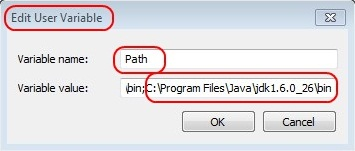
\includegraphics[scale=0.9]{imgs/path_user.jpg}
  \caption{Path to add to the \emph{user} \emph{Path} variable.}
  \label{fig:path_user}
\end{center}
\end{figure}

Note that, figure \ref{fig:path_user} you have to replace \verb=C:\Program Files\Java\jdk1.6.0_26\bin=
for your system's Java bin directory. Also, beware that the environment
variable you have to edit is the \emph{user} Path variable.

\begin{figure}[h]
\begin{center}
  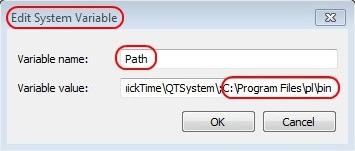
\includegraphics[scale=0.9]{imgs/path_system.jpg}
  \caption{Path to add to the \emph{system} \emph{Path} variable.}
  \label{fig:path_system}
\end{center}
\end{figure}

In figure \ref{fig:path_system}, you have to replace \verb=C:\Program Files\pl\bin= for your prolog installation
bin directory too. This time the variable to edit is the \emph{System} Path
variable.

\begin{figure}[h]
\begin{center}
  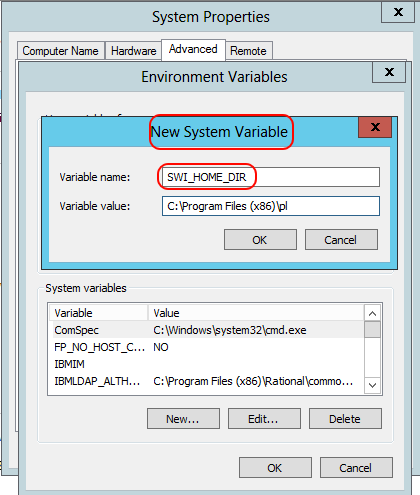
\includegraphics[width=0.6\textwidth]{imgs/swi_prolog_path.png}
  \caption{Path to add to the \emph{system} \emph{SWI\_HOME\_DIR} variable.}
  \label{fig:swi_pl_path}
\end{center}
\end{figure}

In figure \ref{fig:path_system}, you have to replace \verb=C:\Program Files (x86)\pl= for your prolog installation
directory.

Now you have to copy the \verb=jpl.jar= file, in the 
\verb=C:\Program Files\pl\lib= 
directory, and paste it in Java's lib directory: 
\verb=C:\Program Files\Java\jdk1.6.0_26\lib=.

\begin{figure}[h]
\begin{center}
  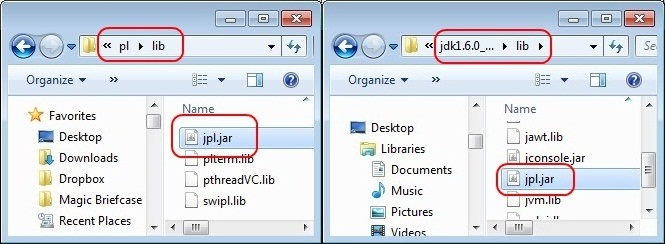
\includegraphics[width=0.8\textwidth]{imgs/jpl_cpy.jpg}
  \caption{Prolog's jpl.jar copied to Java's lib directory.}
  \label{fig:jpl_cpy}
\end{center}
\end{figure}

Finally, you need to install the DSLTrans plugins, placing them in the
eclipse plugins directory (e.g., \verb=C:\Users\clagms\Desktop\eclipse\plugins=)


\begin{figure}[h]
\begin{center}
  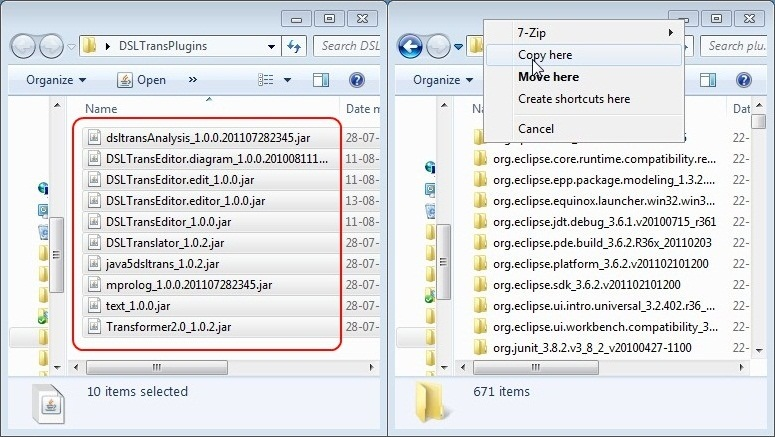
\includegraphics[width=\textwidth]{imgs/dsltrans_plugins_cpy.jpg}
  \caption{DSLTrans plugins being copied to eclipse's plugins directory.}
  \label{fig:dsltrans_plugins_cpy}
\end{center}
\end{figure}

\clearpage


\begin{comment}	

Download & Install Prolog

Download & Install Plugins

Handle java library path

Path do admin com C:\Program Files\pl\bin

Copy jpl.jar to lib java folder

\end{comment}



% \subsection{Linux}
% TODO